% SPDX-License-Identifier: Apache-2.0
% TEXSTAGE FEATURE SHOWCASE: A picnic, planned together
% Runnable slides and brief feature notes are in this main file.
% texstage present examples/showcase/showcase.tex --no-tunnel
% README.md: setup. COVERAGE.md: feature map.
\documentclass[aspectratio=169,11pt]{beamer}
\usepackage{texquiz} % loads texstage.sty, the shared core
\usepackage{texvideo}
\usepackage{texactivity}
\usepackage{booktabs}
\usetikzlibrary{arrows.meta,positioning}
\definecolor{picnicgreen}{HTML}{176B57}
\definecolor{picnicink}{HTML}{183A43}
\definecolor{picnicgold}{HTML}{DDAA37}
\definecolor{picniclight}{HTML}{EAF4EE}
\setbeamercolor{structure}{fg=picnicgreen}
\setbeamercolor{normal text}{fg=picnicink,bg=white}
\setbeamercolor{frametitle}{fg=picnicgreen}
\setbeamerfont{frametitle}{size=\Large,series=\bfseries}
\setbeamertemplate{navigation symbols}{}
\setbeamertemplate{footline}{\hfill\usebeamercolor[fg]{structure}\scriptsize
  texstage showcase\quad\insertframenumber\hspace{5mm}\vspace{3mm}}
\setbeamersize{text margin left=9mm,text margin right=9mm}
% Representative customization; the reference documents every label and theme hook.
\quizsetup{time=45,points=standard,leaderboard=false,shuffle=false,
  title={Let's decide},join-title={Join our picnic},
  leaderboard-title={How are we doing?},podium-title={Thanks for taking part!},
  join-text={Open the presenter-supplied address on your phone and enter the PIN.}}
\renewcommand{\texquizchoicefont}{\normalsize}
\newcommand{\say}[1]{{\Large #1}\par}
\newcommand{\smallgap}{\par\vspace{4mm}}
\newcommand{\codeexample}[1]{{\small\ttfamily #1}\par}
\title{A picnic, planned together}
\subtitle{A guided tour of texstage}
\author{A demonstration with fictional people and data}
\date{}
\begin{document}
% EXAMPLE 01: presenter, projector, notes, recording
\begin{frame}[label=welcome]{A picnic, planned together}
  \vspace{4mm}
  {\huge\bfseries A small plan.\par A room full of ideas.}\par
  \vspace{7mm}
  \say{Let's turn a LaTeX presentation into a shared experience.}
  \smallgap Questions, drawings, video and live activities with texstage.
  \note{Feature example: presenter, projector, notes, recording. These notes are visible in the presenter view.}
\end{frame}
% EXAMPLE 02: explain the product
\begin{frame}{One source connects three views}
  \centering
  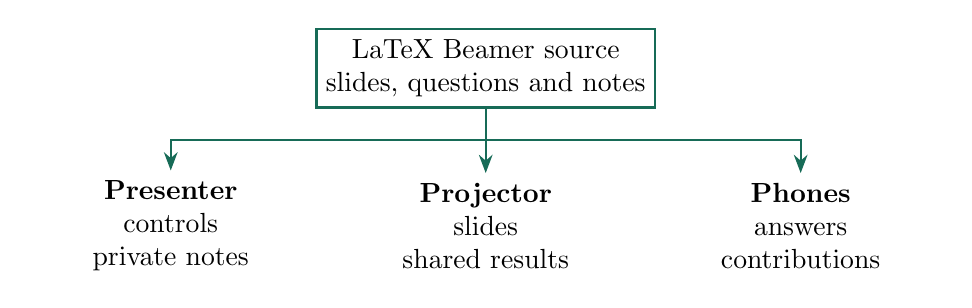
\begin{tikzpicture}[every node/.style={align=center},>=Stealth]
    \node[draw=picnicgreen,thick,minimum width=4cm,minimum height=1cm] (src) at (0,2) {LaTeX Beamer source\\slides, questions and notes};
    \node[text width=3.4cm] (p) at (-4,0) {\textbf{Presenter}\\controls\\private notes};
    \node[text width=3.4cm] (s) at (0,0) {\textbf{Projector}\\slides\\shared results};
    \node[text width=3.4cm] (f) at (4,0) {\textbf{Phones}\\answers\\contributions};
    \draw[->,thick,picnicgreen] (src.south) -- ++(0,-.4) -| (p.north);
    \draw[->,thick,picnicgreen] (src.south) -- (s.north);
    \draw[->,thick,picnicgreen] (src.south) -- ++(0,-.4) -| (f.north);
  \end{tikzpicture}
  \smallgap \say{Participants open a link. They do not install LaTeX.}
  \note{Feature example: explain the product. These notes are visible in the presenter view.}
\end{frame}
% EXAMPLE 03: ordinary Beamer overlays, outside quiz frames
\begin{frame}{Our picnic needs three decisions}
  \begin{enumerate}
    \item<1-> Choose a meeting place.
    \item<2-> Pack what we need.
    \item<3-> Share jobs and ideas.
  \end{enumerate}
  \smallgap \uncover<4->{\say{Everyone can help, even from the back row.}}
  \note{Feature example: ordinary Beamer overlays, outside quiz frames. These notes are visible in the presenter view.}
\end{frame}
% EXAMPLE 04: join, PIN, QR and reconnect
\quizjoinframe[title={Join our picnic},note={Feature example: join, PIN, QR and reconnect. These notes are visible in the presenter view.}]
% EXAMPLE 05: single-selection poll
\begin{quiz}[id=place,type=poll,select=single,cols=3]{Where would you like to sit?}
  \choice[id=meadow]{Open meadow}
  \choice[id=shade]{Under the trees}
  \choice[id=lake]{Beside the lake}
  \note{Feature example: single-selection poll. These notes are visible in the presenter view.}
\end{quiz}
% EXAMPLE 06: ink, laser, zoom, navigation and display controls
\begin{frame}[label=map]{We will meet at the gate at 12:00}
  \begin{columns}[T,onlytextwidth]
  \column{.70\textwidth}
  \centering
  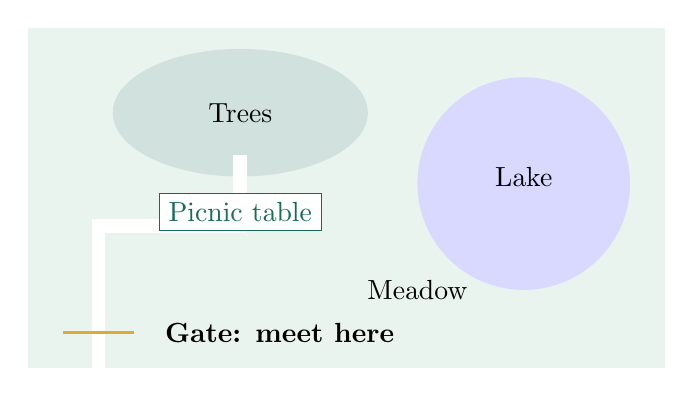
\begin{tikzpicture}[x=.9cm,y=.9cm]
    \fill[picniclight] (0,0) rectangle (9,4.8);
    \fill[blue!15] (7,2.6) ellipse (1.5 and 1.5);
    \node at (7,2.7) {Lake};
    \fill[picnicgreen!20] (3,3.6) ellipse (1.8 and .9);
    \node at (3,3.6) {Trees};
    \node at (5.5,1.1) {Meadow};
    \draw[line width=5pt,white] (1,0)--(1,2)--(3,2)--(3,3);
    \draw[very thick,picnicgold] (.5,.5)--(1.5,.5);
    \node[anchor=west] at (1.8,.5) {\textbf{Gate: meet here}};
    \node[draw,picnicgreen,fill=white] at (3,2.2) {Picnic table};
  \end{tikzpicture}
  \column{.27\textwidth}
  \textbf{Our plan}\par\smallgap
  Meet at the gate.\par\smallgap Walk to the trees.\par\smallgap Keep the path clear.
  \end{columns}
  \note{Feature example: ink, laser, zoom, navigation and display controls. These notes are visible in the presenter view.}
\end{frame}
% EXAMPLE 07: single choice, stable IDs, shuffle and automatic leaderboard
\begin{quiz}[id=meeting,type=single,shuffle,cols=2,time=30,leaderboard=true]{Where do we meet at 12:00?}
  \choice[id=lake]{At the lake}
  \choice*[id=gate]{At the gate}
  \choice[id=table]{At the picnic table}
  \choice[id=meadow]{In the meadow}
  \explain{Meet at the gate first. Then walk to the trees together.}
  \note{Feature example: single choice, stable IDs, shuffle and automatic leaderboard. These notes are visible in the presenter view.}
\end{quiz}
% EXAMPLE 08: multiple choice, partial credit, double points
\begin{quiz}[id=reuse,type=multiple,partial,points=double,cols=2]{Which two items can we use again next time?}
  \choice*[id=bottle]{Refillable bottle}
  \choice*[id=cup]{Washable cup}
  \choice[id=wrapper]{Used snack wrapper}
  \choice[id=napkin]{Used paper napkin}
  \explain{Wash and reuse the bottle and cup. This round allows partial credit and double points.}
  \note{Feature example: multiple choice, partial credit, double points. These notes are visible in the presenter view.}
\end{quiz}
% EXAMPLE 09: true / false
\begin{quiz}[id=budget,type=truefalse,answer=true]{Six people paying 4 euros each give us 24 euros.}
  \explain{Yes: $6 \times 4 = 24$. Everyone contributes the same amount.}
  \note{Feature example: true / false. These notes are visible in the presenter view.}
\end{quiz}
% EXAMPLE 10: decimal slider, tolerance, units
\begin{quiz}[id=water,type=numeric,answer=0.25,tolerance=0.01,min=0,max=1,step=0.05,unit={L}]{Share 1.5 litres equally into six cups. How much goes in each?}
  \explain{$1.5 \div 6 = 0.25$ litres per cup. The accepted tolerance is 0.01 litres.}
  \note{Feature example: decimal slider, tolerance, units. These notes are visible in the presenter view.}
\end{quiz}
% EXAMPLE 11: numeric entry without slider
\begin{quiz}[id=plates,type=numeric,answer=6]{One plate for each of six people. How many plates?}
  \explain{We need six plates. Without slider bounds, the phone uses a number field.}
  \note{Feature example: numeric entry without slider. These notes are visible in the presenter view.}
\end{quiz}
% EXAMPLE 12: numeric estimate without an answer key
\begin{quiz}[id=duration,type=numeric,min=30,max=180,step=15,unit={min}]{How long would you like to stay?}
  \note{Feature example: numeric estimate without an answer key. These notes are visible in the presenter view.}
\end{quiz}
% EXAMPLE 13: text aliases and delayed answer
\begin{quiz}[id=blanket,type=text,reveal=none,time=40]{What large cloth could we spread on the grass to sit on?}
  \accept{blanket}
  \accept{picnic blanket}
  \note{Feature example: text aliases and delayed answer. These notes are visible in the presenter view.}
\end{quiz}
\begin{frame}{A short pause before the answer}
  \say{Think of something that folds into a bag\\and gives us room to sit together.}
  \smallgap We can discuss our guesses before revealing the answer.
  \note{Feature example: text aliases and delayed answer. These notes are visible in the presenter view.}
\end{frame}
\begin{frame}[answer=blanket]{A picnic blanket}
  \say{A \textbf{blanket} gives us a shared place to sit.}
  \smallgap This example accepts both \emph{blanket} and \emph{picnic blanket}.
  \note{Feature example: text aliases and delayed answer. These notes are visible in the presenter view.}
\end{frame}
% EXAMPLE 14: ordering and explicitly placed standings
\begin{quiz}[id=sequence,type=order,partial]{Put our picnic steps in order.}
  \step{Agree on a place and time}
  \step{Pack the picnic bag}
  \step{Meet and enjoy the picnic}
  \step{Clear up before leaving}
  \explain{Make the plan, prepare, enjoy it, then leave the place tidy.}
  \note{Feature example: ordering and explicitly placed standings. These notes are visible in the presenter view.}
\end{quiz}
\quizleaderboardframe[note={Feature example: ordering and explicitly placed standings. These notes are visible in the presenter view.}]
% EXAMPLE 15: multi-select poll, word cloud and free text list
\begin{quiz}[id=games,type=poll,select=multiple,cols=3]{Which activities would you enjoy? Choose any.}
  \choice{A short walk}
  \choice{A card game}
  \choice{Conversation}
  \note{Feature example: multi-select poll, word cloud and free text list. These notes are visible in the presenter view.}
\end{quiz}
\begin{quiz}[id=mood,type=open,display=wordcloud,max-chars=30]{In one word, what makes a good picnic?}
  \note{Feature example: multi-select poll, word cloud and free text list. These notes are visible in the presenter view.}
\end{quiz}
\begin{quiz}[id=welcome-ideas,type=open,display=list,max-chars=160]{What could make our picnic more welcoming?}
  \note{Feature example: multi-select poll, word cloud and free text list. These notes are visible in the presenter view.}
\end{quiz}
% EXAMPLE 16: drawing and sketch gallery
\begin{quiz}[id=table-plan,type=sketch,time=90]{Draw the picnic table from above. Leave a clear path beside it.}
  \note{Feature example: drawing and sketch gallery. These notes are visible in the presenter view.}
\end{quiz}
% EXAMPLE 17: actual local video, poster, trimming, loop, muted playback
\begin{frame}{Our bag is almost ready}
  \centering
  \video[id=packing,poster=packing-poster.jpg,width=.78\linewidth,
    start=1,end=8,loop,muted]{packing.mp4}
  \note{Feature example: actual local video, poster, trimming, loop, muted playback. These notes are visible in the presenter view.}
\end{frame}
% EXAMPLE 18: Q\&A and spontaneous polls
\begin{frame}{What do we still need to know?}
  \say{Ask a question or vote for someone else's question.}
  \smallgap Example: Where can we refill our bottles?
  \note{Feature example: Q\&A and spontaneous polls. These notes are visible in the presenter view.}
\end{frame}
\begin{frame}{One quick decision before we leave}
  \say{Should we take a card game?}
  \smallgap A question raised during the talk can become a live poll.
  \note{Feature example: Q\&A and spontaneous polls. These notes are visible in the presenter view.}
\end{frame}
% EXAMPLE 19: three-field tuples, manual opening, review, loose terms
\begin{frame}[t]{Who will bring what?}
  \begin{activity}[id=bring,input=tuple,fields={Person,Action,Item},
    suggest={Alex,Sam,Riley,brings,apples,water,blanket},
    open=manual,review,terms=loose,min=1,limit=3,height=.57\textheight]
    \prompt{Add a contribution such as Alex / brings / apples.}
  \end{activity}
  \note{Feature example: three-field tuples, manual opening, review, loose terms. These notes are visible in the presenter view.}
\end{frame}
% EXAMPLE 20: two-field tuples, automatic opening, exact terms, minimum agreement
\begin{frame}[t]{Who can carry the table together?}
  \begin{activity}[id=carry,input=tuple,fields={Person,Partner},
    suggest={Alex,Sam,Riley},open=auto,terms=exact,min=2,limit=2,height=.57\textheight]
    \prompt{Suggest a pair: Alex / Sam. Two participants must support the same pair.}
  \end{activity}
  \note{Feature example: two-field tuples, automatic opening, exact terms, minimum agreement. These notes are visible in the presenter view.}
\end{frame}
% EXAMPLE 21: plain-language setup for code activities
\begin{frame}{Our fixed packing list for the next examples}
  \begin{columns}[T,onlytextwidth]
    \column{.46\textwidth}\large
    \begin{tabular}{lr}
      \toprule Item & Quantity\\\midrule
      Apples & 6\\Cups & 6\\Blankets & 2\\\bottomrule
    \end{tabular}
    \column{.49\textwidth}
    \say{Which items have a quantity of six?}
    \smallgap We expect \textbf{Apples} and \textbf{Cups}.
  \end{columns}
  \smallgap The next activities include ready-to-copy examples.
  No coding experience is needed to follow the story.
  \note{Feature example: plain-language setup for code activities. These notes are visible in the presenter view.}
\end{frame}
% EXAMPLE 22: SQL, inline seed/reference, token buttons, result groups
\begin{frame}[t,fragile]{Ask the packing list with SQL}
  \codeexample{SELECT item FROM packing WHERE quantity = 6;}
  \begin{activity}[id=packing-sql,input=code,engine=sql,
    tokens={SELECT,FROM,WHERE,quantity},limit=5,height=.48\textheight]
    \prompt{Return the items with quantity 6. Try the query above.}
    \seed{CREATE TABLE packing (item TEXT, quantity INTEGER);
INSERT INTO packing VALUES ('Apples',6),('Cups',6),('Blankets',2);}
    \reference{SELECT item FROM packing WHERE quantity = 6;}
  \end{activity}
  \note{Feature example: SQL, inline seed/reference, token buttons, result groups. These notes are visible in the presenter view.}
\end{frame}
% EXAMPLE 23: explain graph data
\begin{frame}{The same plan can be written as facts}
  \say{Alex brings apples.}\smallgap
  \say{Sam brings water.}\smallgap
  \say{Riley brings a blanket.}
  \vspace{7mm} A graph connects each person to the item they bring.
  \note{Feature example: explain graph data. These notes are visible in the presenter view.}
\end{frame}
% EXAMPLE 24: SPARQL, file seed/reference and manual opening
\begin{frame}[t,fragile]{Ask the graph with SPARQL}
  \codeexample{SELECT ?person WHERE \{ ?person :brings :water . \}}
  \begin{activity}[id=water-sparql,input=code,engine=sparql,seed=picnic.ttl,
    reference=water.rq,tokens={SELECT,WHERE,:brings,:water},
    open=manual,limit=4,height=.48\textheight]
    \prompt{Who brings water? Try the query above. We expect Sam.}
  \end{activity}
  \note{Feature example: SPARQL, file seed/reference and manual opening. These notes are visible in the presenter view.}
\end{frame}
% EXAMPLE 25: Turtle graph comparison
\begin{frame}[t,fragile]{Add one fact with Turtle}
  \codeexample{:Sam :brings :bread .}
  \begin{activity}[id=bread-turtle,input=code,engine=turtle,seed=picnic.ttl,
    reference=bread.ttl,tokens={:Sam,:brings,:bread,.},limit=4,height=.48\textheight]
    \prompt{Write the fact: Sam brings bread. Include the final dot.}
  \end{activity}
  \note{Feature example: Turtle graph comparison. These notes are visible in the presenter view.}
\end{frame}
% EXAMPLE 26: whiteboards and optional paired tablet
\begin{frame}{Our final shared checklist}
  \say{Meeting place agreed.}\smallgap
  \say{Food and equipment assigned.}\smallgap
  \say{Space left for everyone's ideas.}
  \note{Feature example: whiteboards and optional paired tablet. These notes are visible in the presenter view.}
\end{frame}
% EXAMPLE 27: hyperlinks and final standings
\begin{frame}{We have a plan}
  \say{Meet at the gate at 12:00.}
  \smallgap Sit under the trees, share the supplies and leave the area tidy.\par
  \vspace{7mm}
  \hyperlink{map}{\beamerbutton{Revisit our map}}\qquad
  \href{https://www.latex-project.org/}{\beamerbutton{About LaTeX}}
  \note{Feature example: hyperlinks and final standings. These notes are visible in the presenter view.}
\end{frame}
\quizpodiumframe[note={Feature example: hyperlinks and final standings. These notes are visible in the presenter view.}]
% EXAMPLE 28: outputs and recording
\begin{frame}{One source, several useful results}
  \begin{itemize}
    \item A live browser presentation with phone participation.
    \item A handout and a separate solutions PDF.
    \item PowerPoint exports for compatible presentation setups.
    \item After the session: annotated slides, results and recordings.
  \end{itemize}
  \smallgap \say{The content stays in a readable LaTeX file.}
  \note{Feature example: outputs and recording. These notes are visible in the presenter view.}
\end{frame}
% EXAMPLE 29: operations that cannot be activated by a static .tex file
\appendix
\begin{frame}{Behind the scenes: prepare the next session}
  \begin{itemize}
    \item Find a deck in the library or upload a bundle.
    \item Resume a presentation or start a new one.
    \item Pair or revoke a presenter device.
    \item Start a fresh quiz game for a new group.
  \end{itemize}
  \smallgap Save session results before starting a new session.
  \note{Feature example: operations that cannot be activated by a static .tex file. These notes are visible in the presenter view.}
\end{frame}
% EXAMPLE 30: deployment/platform boundaries
\begin{frame}{Choose the setup for your audience}
  \begin{tabular}{@{}p{.25\linewidth}p{.66\linewidth}@{}}
    \toprule
    Browser & Complete tour, including activities and presenter tools.\\[2mm]
    PowerPoint & Static export, or supported live quiz/video integration with setup.\\[2mm]
    Local or hosted & Reachable address for phones; HTTPS for remote use.\\
    \bottomrule
  \end{tabular}
  \smallgap Installation instructions and the feature checklist accompany this source.
  \note{Feature example: deployment/platform boundaries. These notes are visible in the presenter view.}
\end{frame}
\end{document}
